% subsection: 特性方程式型 \, $a_{n+1}=pa_n+q$

\subsection{\texorpdfstring{特性方程式型  $a_{n+1}=pa_n+q$}{特性方程式型}}\label{節：特性方程式型}
  本節の流れだが,まずはメジャーな解法を解説する.
  解説の後に例題とその解説等があり,その後で,解法の詳細な発想や原理,別解などを扱う.
  
  では本題に入ろう.
  まず,諸君らは,基本4パターンであればこれまでの知識を使って解くことができる.
  したがって特性方程式型漸化式を基本パターンのいずれかの形に変形して一般項を得ることを目標とする.
  
  結論から言えば漸化式を等比数列に変形することで,一般項を得ることができる.
  また,多くの複雑な漸化式は等比型に帰着させることでその解を得る.\footnote{基本的に等比型,特性方程式型,定数数列への帰着が多い.既知のパターンを増やしていくことが解ける漸化式を増やすためには重要である.}
  等比型にするためには$q$が邪魔なので,それをうまく消せるように
  \[
    \begin{array}{rrl}
      &a_{n+1}={}&pa_n+q\\
      -\,)&\alpha={}&p\alpha+q\\ \hline
      &a_{n+1}-\alpha={}&p(a_n-\alpha)
    \end{array}
  \]
  という式を考える.
  これによって$b_n=a_n-\alpha$という$b_n$に関する等比型漸化式が得られる.
  あとは$\alpha$について
  \[
    \alpha=p\alpha+q
  \]
  を解き,
  \[
    a_{n+1}-\alpha=p(a_n-\alpha)
  \]
  とすることで等比型に帰着させることで一般項を得る.

  形式的には,$a_n$を$\alpha$に置き換えてできる方程式によってその解を得れば良い.
  また,方程式
  \[
    \alpha=p\alpha+q
  \]
  を特性方程式という.\footnote{\chapterref{章：付録}では,特性方程式を中心に線形代数の考えを導入して他の漸化式の解法と統一的な見方を分析する.}

  これだけの説明では納得できない読者は例題の後に続く部分を読むと良い.

  \begin{bookpoint}
    \textbf{POINT}\par
    特性方程式$\alpha=p\alpha+q$を解いて$a_{n+1}-\alpha=p(a_n-\alpha)$として等比型に帰着させる.
  \end{bookpoint}
  \noindent \bookblocklink{example-characteristic-1}{problem}{answer}{【例題】}\par\nobreak
  \begin{enumerate}[label=(\arabic*),parsep=3pt,format=\bookitemlink{example-characteristic-1}{problem}{answer}]
    \item $\displaystyle a_1=1,\, a_{n+1}=2a_n+1$
    \item $\displaystyle a_1=1,\, a_{n+1}=\frac{1}{2}a_n+2$
    \item $\displaystyle a_1=1,\, a_{n+1}=a_n+2$
  \end{enumerate}
  
  \noindent\bookblocklink{example-characteristic-1}{hint}{problem}{【方針】}\par\nobreak
  \begin{enumerate}[label=(\arabic*),parsep=3pt,format=\bookitemlink{example-characteristic-1}{hint}{problem}]
    \item まずは,$\alpha$を求めて等比型に帰着させる方法で解きましょう.
    \item 同じく,$\alpha$を求めて等比型に帰着させる方法で解きましょう.
    \item 等差型として解けます.定数を引く方法では,$\alpha=\alpha+2$を満たす値がないことも確かめましょう.
  \end{enumerate}
  
  \noindent\bookblocklink{example-characteristic-1}{answer}{problem}{【解答】}\par\nobreak
  \begin{enumerate}[label=(\arabic*),parsep=3pt,format=\bookitemlink{example-characteristic-1}{answer}{problem}]
    \item $\displaystyle a_n=2^n-1$
    \item $\displaystyle a_n=4-3\cdot\left(\frac{1}{2}\right)^{n-1}$
    \item $\displaystyle a_n=1+2(n-1)$
  \end{enumerate}
  
  \noindent\bookblocklink{example-characteristic-1}{solution}{problem}{【解法】}\par\nobreak
  \begin{enumerate}[label=(\arabic*),parsep=3pt,format=\bookitemlink{example-characteristic-1}{solution}{problem}]
    \item $\alpha=2\alpha+1$より\bookterm{fixed}{不動点}は$-1$である.$b_n=a_n+1$と置くと,
      \[
        \begin{aligned}
          b_{n+1}&=2(a_n+1)=2b_n,\\
          b_1&=2.
        \end{aligned}
      \]
      従って$b_n=2^n$であり,$a_n=b_n-1=2^n-1$となる.
    \item $\alpha=\frac12\alpha+2$より\bookterm{fixed}{不動点}は$4$である.$b_n=a_n-4$と置くと,
      \[
        \begin{aligned}
          b_{n+1}&=\frac12(a_n-4)=\frac12b_n,\\
          b_1&=-3.
        \end{aligned}
      \]
      従って$b_n=-3(\frac12)^{n-1}$であり,$a_n=4-3(\frac12)^{n-1}$となる.
    \item $\alpha=\alpha+2$を満たす値はなく,定数を引く方法は使えない.
      等差型として$a_n=1+2(n-1)$を得る.
  \end{enumerate}

  \subsubsection{式変形の発想}
  まずは漸化式を眺めてみよう.
  \[
   a_{n+1}=pa_n+q
  \]
  この漸化式は,いわば等差型と等比型が組み合わさったような漸化式である.\footnote{ただし$p=1$なら等差型であり,$p=0$なら直接$n\ge2$で$a_n=q$と分かる.}
  解き方を模索する際にはまず実験を行うのが常套である.
  $p,q$に適当な値を代入して第10項程度まで求めてみると
  \begin{table}[htbp]
    \rowcolors{2}{black!10}{white}
    \begin{tabular}{cccc}\Xhline{1.5pt}
      n&	$p=2,\,q=1$&	$p=4,\,q=1$&	$p=2,\,q=10$\\
      1&	1&	1&	1\\
      2&	3&	5&	12\\
      3&	7&	21&	34\\
      4&	15&	85&	78\\
      5&	31&	341&	166\\
      6&	63&	1365&	342\\
      7&	127&	5461&	694\\
      8&	255&	21845&	1398\\
      9&	511&	87381&	2806\\
      10&	1023&	349525&	5622\\
    \end{tabular}
  \end{table}
  となる.グラフにしてみると
   
  \begin{figure}[htbp]
    \centering
    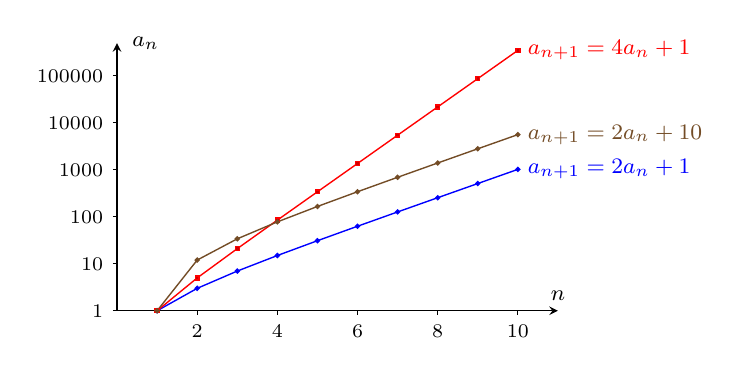
\begin{tikzpicture}
      \begin{axis}[
          scale only axis,
          width=5.6cm,
          height=3.4cm,                     % 高さを抑える(旧 4.8cm)
          clip=false,                       % 線の先の式をはみ出して表示
          % --- 軸(矢印つき・枠なし・モノクロ) ---
          axis lines=left,
          axis line style={->,>=stealth,thin,black},
          ymode=log,
          xmin=0, xmax=11,
          ymin=1, ymax=500000,
          xtick={2,4,6,8,10},
          ytick={1,10,100,1000,10000,100000},
          yticklabels={1,10,100,1000,10000,100000},
          tick align=outside,
          major tick length=1.5pt,
          minor tick length=0pt,
          tick style={black,thin},
          tick label style={font=\scriptsize,black},
          % --- 線・点(すべて黒、細く小さく) ---
          every axis plot/.append style={
            black, line width=0.5pt,
            mark=*, mark size=0.7pt, mark options={solid,fill=black},
          },
        ]
        % 軸ラベル
        \node[above]     at (rel axis cs:1,0) {\footnotesize $n$};
        \node[right=2pt] at (rel axis cs:0,1) {\footnotesize $a_n$};
   
        % p=2, q=1
        \addplot coordinates {
          (1,1) (2,3) (3,7) (4,15) (5,31)
          (6,63) (7,127) (8,255) (9,511) (10,1023)
        } node[pos=1,right,font=\footnotesize] {$a_{n+1}=2a_n+1$};
   
        % p=4, q=1
        \addplot coordinates {
          (1,1) (2,5) (3,21) (4,85) (5,341)
          (6,1365) (7,5461) (8,21845) (9,87381) (10,349525)
        } node[pos=1,right,font=\footnotesize] {$a_{n+1}=4a_n+1$};
   
        % p=2, q=10
        \addplot coordinates {
          (1,1) (2,12) (3,34) (4,78) (5,166)
          (6,342) (7,694) (8,1398) (9,2806) (10,5622)
        } node[pos=1,right,font=\footnotesize] {$a_{n+1}=2a_n+10$};
      \end{axis}
    \end{tikzpicture}
    \caption{$p,q$の値による漸化式が成す値の変化}
  \end{figure}
  
  となる.
  これが対数グラフであることに注意して観察してみると,$p$の値が数列の成す値に関して支配的であることが分かる.
  また,$q$はそこまでグラフの値の変化に大きく影響するわけでないことも分かる.
  実際,$a_n$に対して$p$が掛けられることで$a_{n+1}$が作られるのだから,等比型の一般項のように,$p^n$のような形が一般項に含まれることは比較的想像しやすいだろう.

  等比型漸化式$a_{n+1}=ra_n$の一般項が$a_n=a_1r^{n-1}$であることを思い出すと,一般項に$p^n$が含まれることが想像できる.
  そこで,$q$や$a_1$分の補正を与えてやれば漸化式から一般項を得られると考え,その方法を検討しよう.
  
  $p$に関しておおよその推測がたった今,いかにして$q$を処理するかが争点になってくる.
  今,読者諸君らが持つ技は,等比型,等差型,階差型,階比型の漸化式を解くことといくつかの基本的な計算テクニックであろう.
  基本的な計算テクニックの内,邪魔なもの,つまりは$q$を消すためにはどのような手法があるだろうか.
  邪魔な項を消す場合は以下のような方法がよく用いられる.
  \begin{enumrate}
    \item 同じ値を引く
    \item 別の等式を用意して代入\footnote{\sectionref{節：総和型}ではこの発想が用いられている}
    \item 約分できるような数で割る\footnote{\sectionref{節：分数型}ではある意味でこの亜種のような計算をする}
    \item 平方完成や部分分数分解のようなテクニックでうまく消えるような項を作る
  \end{enumrate}
  平方完成や部分分数分解ができるような複雑な見た目をしていないし,約分しようにも$q$を消す約分をしたところで,問題の本質はそこまで変わらないだろう.\footnote{$\frac{a_{n+1}}{q}=\frac{p}{q}a_{n}+1$となるが,$a_n$が定数倍されたものに定数を足したものが次の項という構造に変化はない.}
  したがって,「同じ値を引く」「別の等式を用意して代入」の2つを試してみよう.
  
  ここからがやっと解法である.
  メジャーな解法は「同じ値を引く」の方なので,先にその方法で示してから,後に「別の等式を用意して代入」の方をお見せしよう.

  \noidnent \textbf{【同じ値を引く】}
  
  結論から述べよう.
  $q$がなくなるように式変形をしてやればよいのだから
  \[
    \begin{array}{rrl}
      &a_{n+1}={}&pa_n+q\\
      -\,)&\alpha={}&p\alpha+q\\ \hline
      &a_{n+1}-\alpha={}&p(a_n-\alpha)
    \end{array}
  \]
  となるような$\alpha$を考えればよいのだ.
  
  言い換えればある実数$\alpha$によって,
  \begin{aligin*}
    a_{n+1}=pa_n+q \iff a_{n+1}-\alpha=p(a_n-\alpha)
  \end{aligin*}
  となるような$\alpha$が存在しさえしてくれれば,漸化式は等比型に帰着する.
  $\alpha$を求めると
  \begin{aigin*}
    &\alpha=p\alpha+q\\
    &\therefore \quad \alpha=\frac{q}{1-p}
  \end{aligin*}
  その後の計算は$b_n=a_n-\alpha$と置くことでもとの漸化式は公比$p$,初項$a_1-\alpha$の等比型漸化式に帰着する.
  \begin{aligin*}
    &b_{n+1}=pb_n\\
    &\therefore \quad b_n=b_1p^{n-1}\\
    &\therefore \quad a_n=(a_1-\alpha)p^{n-1}+\alpha
    &\therefore \quad a_n=(a_1-\frac{q}{1-p})p^{n-1}+\frac{q}{1-p}
  \end{aligin*}
  以上より一般項を得る.
  
  この式変形の図形的意味を考えてみよう.
  少々突飛な発想だが,
  \[
    a_{n+1}=pa_n+q
  \]
  の式を
  \[
    y=px+q
  \]
  として考えてみよう.
  つまり,$a_n$の値による$a_{n+1}$の値の変化をグラフに落とし込むということだ.
  図示すると
  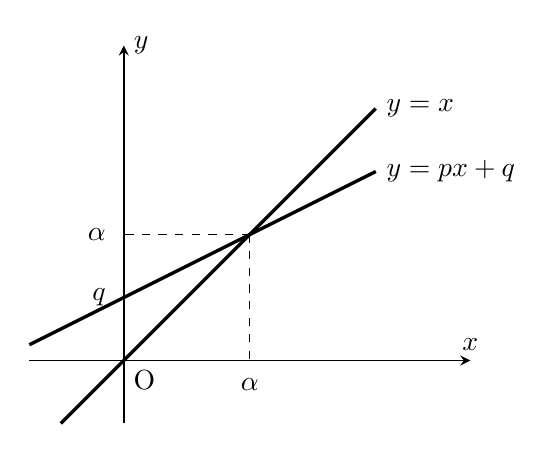
\begin{tikzpicture}[scale=0.8]
    \draw[->,>=stealth,semithick] (-1.5,0)--(5.5,0)node[above]{$x$};
    \draw[->,>=stealth,semithick] (0,-1)--(0,5)node[right]{$y$};
    \draw (0,0)node[below right]{O};
  
    \draw[very thick,domain=-1:4]
    plot(\x,\x)node[right]{$y=x$};
  
    \draw[very thick,domain=-1.5:4]
    plot(\x,\x/2+1) node[right] {$y=px+q$};
  
    % q
    \node[left=3pt] at (0,1) {$q$};
  
    % 交点から各軸へ点線
    \draw[dashed] (2,2) -- (2,0);
    \draw[dashed] (2,2) -- (0,2);
  
    % α
    \node[below=3pt] at (2,0) {$\alpha$};
    \node[left=3pt] at (0,2) {$\alpha$};
  \end{tikzpicture}
  \begin{center}
    \BookFigureCaption{直線の交点として捉える\bookterm{fixed}{不動点}}
  \end{center}

  となる.
  $y=x$のグラフは$a_{n+1}=a_n$という公比1の等比数列としてみなしたときに,これらのグラフの交点を原点と思って漸化式を見直してやれば,点$(\alpha,\alpha)$が原点であるような等比数列となるのだ.

  このような点$(\alpha,\alpha)$を不動点という.
  特性方程式は不動点を求める漸化式で,不動点は特性方程式型漸化式を等比型漸化式としてみなせるようになる(ずらすことで"きれい"にできる)点である.
  
  初項が$\alpha$なら定数解,異なるなら$|p|>1$でずれが増大し,$|p|<1$で$0$へ近づく.
  後者では$a_n\to\alpha$となる.

  \noidnent \textbf{【別の等式を用意して代入】}
  
  同じ$q$を消すには,隣り合う二つの漸化式をを引く方法もある.
  \begin{align*}
    &a_{n+1}=pa_n+q \booktag{affine-difference-1}{♡}\\
    &a_{n+2}=pa_{n+1}+q \booktag{affine-difference-2}{♢}\\
  \end{align*}
  $\bookeqbackref{affine-difference-2}{(♢)}-\bookeqbackref{affine-difference-1}{(♡)}$をし
  \[
    a_{n+2}-a_{n+1}=p(a_{n+1}-a_n)
  \]
  ここで,$d_n=a_{n+1}-a_n$と置くと,
  \[
    d_{n+1}=pd_n,\qquad d_1=(p-1)a_1+q
  \]
  となる.等比型になった\textbf{階差}$d_n=d_1p^{n-1}$を,\sectionref*{節：階差型}と同じように足し戻す.
  \begin{align*}
    a_n&=a_1+\sum_{k=1}^{n-1}d_k\\
    &=a_1+d_1\frac{p^{n-1}-1}{p-1}\\
    &=\alpha+(a_1-\alpha)p^{n-1}
  \end{align*}
  $d_1=(p-1)(a_1-\alpha)$より,不動点を引く方法と一致する.
  $p=1$の場合も階差は一定なので,$a_n=a_1+(n-1)q$と足し戻せる.
  
  二つの直線$y=px$と$y=px+q$の差は$q$である.一方,更新式どうしの引き算では異なる入力を比べる.
  $f(x)=px+q$なら,
  \[
    f(x)-f(y)=(px+q)-(py+q)=p(x-y)
  \]
  となる.$x=a_{n+1},\ y=a_n$としたものが\bookeqref{affine-difference-2}{(2)}から\bookeqref{affine-difference-1}{(1)}を引いた式である.\footnote{添字を一つずらして引く操作は,付録\sectionref{節：和と差から微積分へ}で扱う\bookterm{difference-operator}{差分}の考え方につながる.}
  共通の$q$が消えた.二つの直線も確認しよう.
  
  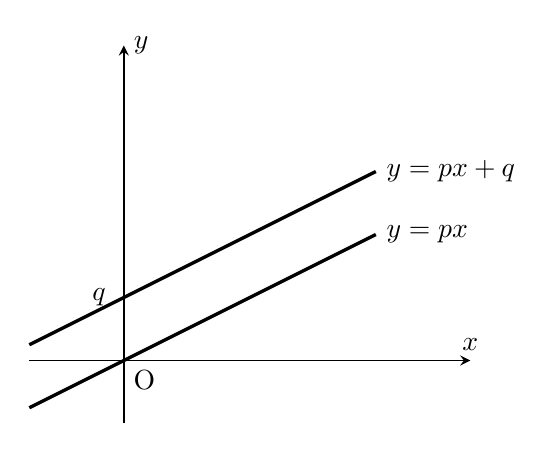
\begin{tikzpicture}[scale=0.8]
    \draw[->,>=stealth,semithick] (-1.5,0)--(5.5,0)node[above]{$x$};
    \draw[->,>=stealth,semithick] (0,-1)--(0,5)node[right]{$y$};
    \draw (0,0)node[below right]{O};
  
    \draw[very thick,domain=-1.5:4]
    plot(\x,\x/2)node[right]{$y=px$};
  
    \draw[very thick,domain=-1.5:4]
    plot(\x,\x/2+1) node[right] {$y=px+q$};
  
    % q
    \node[left=3pt] at (0,1) {$q$};
  
  \end{tikzpicture}
  \begin{center}
    \BookFigureCaption{定数項の違いを表す平行な直線}
  \end{center}
  
  不動点からのずれと隣り合う項の差は,同じ定数項を消す二つの見方である.
  この先では引く量が一次式などへ広がり,二項をまとめる際には倍率を求める\mbox{\bookterm{characteristic}{特性方程式}}が現れる.
  今の$\alpha$は変わらない値,後の根は更新の倍率である.付録の\bookterm{matrix}{行列}でもつながりを見直す.

  \noident \textbf{【$p$へのアプローチ】}
  
  ここまで$q$を消す試みを続けてきたが,$p$にたいしてうまく操作できないだろうか.
  \sectionref{節：階差階比複合型}でも使われる式変形を用いればうまく解くことができる.
  \[
    a_{n+1}=pa_n+q
  \]
  について,$p^{n+1}$で割って,
  \[
    \frac{a_{n+1}}{p^{n+1}}=\frac{a_n}{p^n}+\frac{q}{p^{n+1}}
  \]
  ここで$\displaystyle b_n=\frac{a_n}{p^n}$と置くと
  \[
    b_{n+1}=b_n+\frac{q}{p^{n+1}}
  \]
  となって階差型となる.
